\documentclass[12pt]{article}
\usepackage[english]{babel}
\usepackage[utf8]{inputenc}
\usepackage[T1]{fontenc}
\usepackage{amsmath}
\usepackage{graphicx}
\usepackage[colorinlistoftodos]{todonotes}
\usepackage{listings}
\usepackage{enumitem}
\usepackage{listingsutf8}
\usepackage{xparse}
\usepackage[hmargin=2cm]{geometry}
\usepackage{color} 
\NewDocumentCommand{\codeword}{v}{%
\texttt{\textcolor{blue}{#1}}%
}
\definecolor{codegreen}{rgb}{0,0.6,0}
\definecolor{codegray}{rgb}{0.5,0.5,0.5}
\definecolor{codepurple}{rgb}{0.58,0,0.82}
\definecolor{backcolour}{rgb}{0.95,0.95,0.92} 
\lstdefinestyle{mystyle}{
    backgroundcolor=\color{backcolour},   
    commentstyle=\color{codegreen},
    keywordstyle=\color{magenta},
    numberstyle=\tiny\color{codegray},
    stringstyle=\color{codepurple},
    basicstyle=\footnotesize,
    breakatwhitespace=false,         
    breaklines=true,                 
    captionpos=b,                    
    keepspaces=true,                 
    numbers=left,                    
    numbersep=5pt,                  
    showspaces=false,                
    showstringspaces=false,
    showtabs=false,                  
    tabsize=2
}
\lstset{style=mystyle}
\lstset{inputencoding=utf8/latin1}
%Para mostrar el código bonito 
\lstset{language=C++} 
\lstdefinestyle{customc}{
  belowcaptionskip=1\baselineskip,
  breaklines=true,
  frame=L,
  xleftmargin=\parindent,
  language=C++,
  showstringspaces=false,
  basicstyle=\footnotesize\ttfamily,
  keywordstyle=\bfseries\color{green!40!black},
  commentstyle=\itshape\color{purple!40!black},
  identifierstyle=\color{blue},
  stringstyle=\color{orange},
}

\begin{document}
\begin{titlepage}
\newcommand{\HRule}{\rule{\linewidth}{0.5mm}}
\center
\textsc{\LARGE Universidad de Granada}\\[1.5cm] % Name of your university/college
\textsc{\Large Sistemas concurrenetes y distribuidos}\\[0.5cm] % Major heading such as course name
\HRule \\[0.4cm]
{ \huge \bfseries Seminario 1: Cálculo concurrente de $\pi$}\\[0.4cm] % Title of your document
\HRule \\[1.5cm]
\begin{minipage}{0.4\textwidth}
\begin{flushleft} \large
\emph{Autora:}\\
Elena Merelo Molina \textsc{} % Your name
\end{flushleft}
\end{minipage}
~
\begin{minipage}{0.4\textwidth}
\begin{flushright} \large
\emph{} \\
\textsc{} % Supervisor's Name
\end{flushright}
\end{minipage}\\[2cm]
{\large Septiembre de 2018}\\[2cm] % Date, change the \today to a set date if you want to be precise

\includegraphics[scale=0.5]{../images/logo.jpg}
\vfill % Fill the rest of the page with whitespace
\end{titlepage}


\section{Enunciado de la práctica}
Como actividad se propone copiar la plantilla en ejemplo09.cpp y completar en este archivo la implementación del cálculo concurrente del número $\pi$ . En la salida se presenta el valor exacto de $\pi$ y el calculado de las tres formas: secuencial, concurrente distribuyendo el trabajo entre hebras de manera contigua, y distribuyéndolo entrelazadamente (sirve para verificar si el programa es correcto). Asimismo, el programa imprimirá la duración del cálculo concurrente contiguo, concurrente entrelazado, secuencial y el porcentaje de tiempo
de estos dos últimos respecto del secuencial.

\section{Explicación de mi solución}
Para resolver el problema he usado cuatro funciones. Veámoslas una a una.

\begin{itemize}[wide, nosep, labelindent = 0pt, topsep = 1ex]
\item[\textbf{Cálculo de las sumas parciales de forma contigua}]
\item \verb|double funcion_hebra_contigua( long i )| Función que ejecuta cada hebra: recibe el índice de la hebra (i<n) y evalúa f desde el comienzo del intervalo, m/n (lo que viene siendo el tamaño de un chunk) multiplicado por la hebra que es, hasta el fin. De esta manera cada hebra calcula un bloque: hebra 0 el primer intervalo formado por cuatro subintervalos, hebra 1 los siguientes cuatro, y así.
\begin{lstlisting}
double funcion_hebra_contigua( long i ) {
  double suma_hebra= 0.0;
  for( long j= m/n*i; j< m/n*(i+1); j++)
    suma_hebra += f((j + double(0.5)) /m);

  return suma_hebra/m;
}
\end{lstlisting}
\item[\textbf{Cálculo de las sumas parciales de forma entrelazada}]
\item \verb|double funcion_hebra_entrelazada( long i )| Función que ejecuta cada hebra: recibe i==índice de la hebra (i<n) y evalúa f desde el comienzo del subintervalo, i, hasta m, el final, dando saltos de n en n, el número de hebras. Consecuentemente, cada hebra calcula un subintervalo: hebra 1 el primero, hebra 2 el segundo,... hebra 1 el quinto, y así sucesivamente.
\begin{lstlisting}
double funcion_hebra_entrelazada( long i ) {
  double suma_hebra= 0.0;
  for( long j= i; j< m ; j += n)
    suma_hebra += f((j + double(0.5)) /m);;

  return suma_hebra/m;
}
\end{lstlisting}
\item[\textbf{Cálculo concurrente de $\pi$ de forma contigua}]
\item \verb|double calcular_integral_concurrente_contigua( )| Calcula la integral de forma concurrente. Una vez las hebras han calculado las sumas parciales de los valores de f, la hebra principal las recoge en una suma total,
repartiendo los bloques entre las hebras de manera contigua.
\begin{lstlisting}
double calcular_integral_concurrente_contigua( ) {
  double suma= 0.0;
  future<double> futuros[n];

  //Ponemos en marcha todas las hebras y obtenemos los futuros
  for( long i= 0; i< n; i++)
    futuros[i] = async( launch::async, funcion_hebra_contigua, i);
  //Esperamos a que cada hebra termine y vamos obteneniendo el resultado de la integral
  for(long i= 0; i<n; i++)
    suma += futuros[i].get();

  return suma;
}
\end{lstlisting}
\item[\textbf{Cálculo concurrente de $\pi$ de forma entrelazada}]
\item \verb|double calcular_integral_concurrente_entrelazada( )| Calcula la integral de forma concurrente. Una vez las hebras han calculado las sumas parciales de los valores de f, la hebra principal las recoge en una suma total,
repartiendo los bloques entre las hebras de manera entrelazada.
\begin{lstlisting}
double calcular_integral_concurrente_entrelazada( ) {
  double suma= 0.0;
  future<double> futuros[n];

  //Ponemos en marcha todas las hebras y obtenemos los futuros
  for( long i= 0; i< n; i++)
    futuros[i] = async( launch::async, funcion_hebra_entrelazada, i);
  //Esperamos a que cada hebra termine y vamos obteneniendo el resultado de la integral
  for(long i= 0; i<n; i++)
    suma += futuros[i].get();

  return suma;
}
\end{lstlisting}

\end{itemize}

\section{Medición de tiempos}
De ello se ocupa el programa principal: 
\begin{lstlisting}
int main() {
  time_point<steady_clock> inicio_sec  = steady_clock::now() ;
  const double             result_sec  = calcular_integral_secuencial(  );
  time_point<steady_clock> fin_sec     = steady_clock::now() ;

  double x = sin(0.4567);
  time_point<steady_clock> inicio_conc_ent = steady_clock::now() ;
  const double             result_conc_ent = calcular_integral_concurrente_entrelazada(  );
  time_point<steady_clock> fin_conc_ent    = steady_clock::now() ;

  time_point<steady_clock> inicio_conc_cont = steady_clock::now() ;
  const double             result_conc_cont = calcular_integral_concurrente_contigua(  );
  time_point<steady_clock> fin_conc_cont   = steady_clock::now() ;

  duration<float,milli>    tiempo_sec  = fin_sec  - inicio_sec ,
                           tiempo_conc_ent = fin_conc_ent - inicio_conc_ent,
                           tiempo_conc_cont= fin_conc_cont - inicio_conc_cont;
  const float              porc_ent        = 100.0*tiempo_conc_ent.count()/tiempo_sec.count(),
                           porc_cont       = 100.0*tiempo_conc_cont.count()/tiempo_sec.count();


  constexpr double pi = 3.14159265358979323846l ;

  cout << "Número de muestras (m)   : " << m << endl
       << "Número de hebras (n)     : " << n << endl
       << setprecision(18)
       << "Valor de PI              : " << pi << endl
       << "Resultado secuencial     : " << result_sec  << endl
       << "Resultado concurrente entrelazada   : " << result_conc_ent << endl
       << "Resultado concurrente contigua   : " << result_conc_cont << endl
       << setprecision(5)
       << "Tiempo secuencial        : " << tiempo_sec.count()  << " milisegundos. " << endl
       << "Tiempo concurrente entrelazada      : " << tiempo_conc_ent.count() << " milisegundos. " << endl
       << "Tiempo concurrente contigua      : " << tiempo_conc_cont.count() << " milisegundos. " << endl
       << setprecision(4)
       << "Porcentaje t.conc_entrelazada/t.sec. : " << porc_ent << "%" << endl
       << "Porcentaje t.conc_contigua/t.sec. : " << porc_cont << "%" << endl;
}

\end{lstlisting}

Al ejecutarlo, resulta: 
\begin{figure}[h]
	\centering
	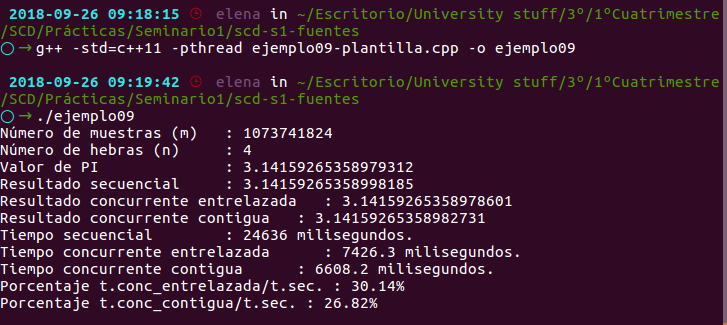
\includegraphics[scale=0.5]{../images/1.png}
	\caption{Resultado de la ejecución}
\end{figure}

Observamos cómo el cálculo concurrente entrelazado produce un número $\pi$ más cercano al real, seguido del contiguo y por último el secuencial, que es más inexacto. No obstante, el cálculo contiguo tarda menos que el entrelazado, y como cabía esperar el secuencial es el más lento.

En la siguiente imagen vemos (en un sistema Ubuntu 16 con 4 CPUs) cómo van evolucionando los porcentajes de uso de cada CPU a lo largo de la ejecución del programa con 4 hebras (es una captura de pantalla del system monitor):
\begin{figure}[h]
	\centering
	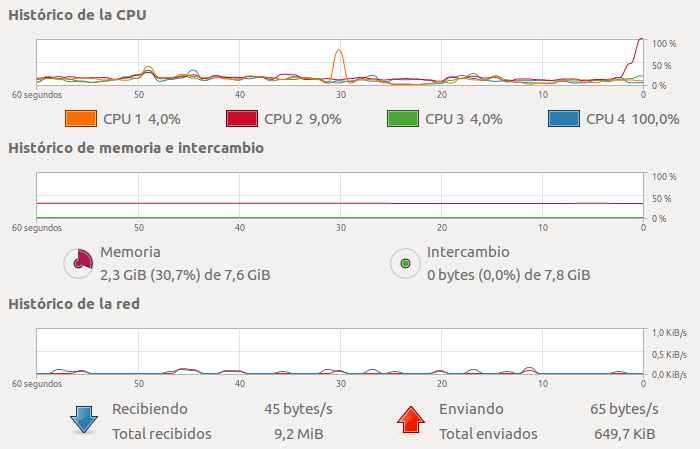
\includegraphics[scale=0.5]{../images/2.png}
	\caption{Inicio de la ejecución}
\end{figure}
\begin{figure}[h]
	\centering
	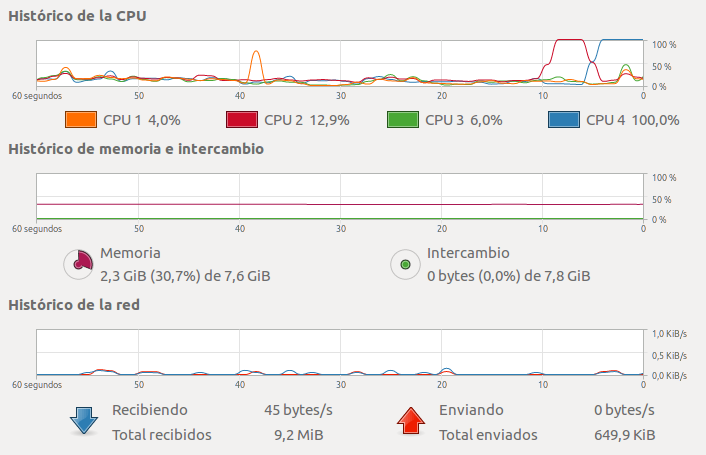
\includegraphics[scale=0.5]{../images/3.png}
	\caption{Comienza parte secuencial}
\end{figure}
\begin{figure}[h]
	\centering
	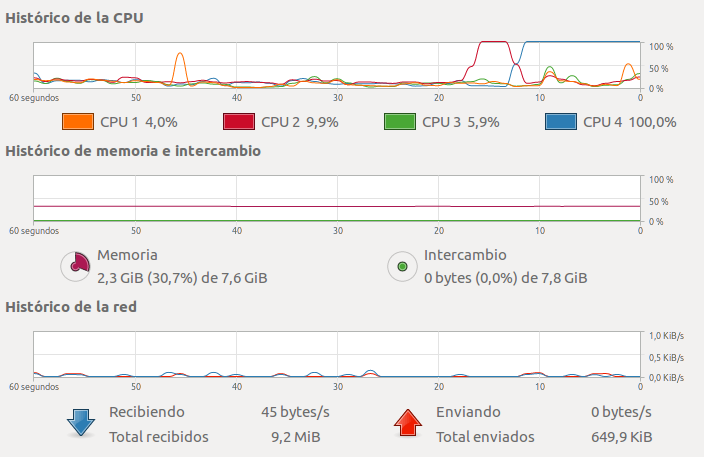
\includegraphics[scale=0.5]{../images/4.png}
	\caption{Continúa parte secuencial}
\end{figure}
\begin{figure}[h]
	\centering
	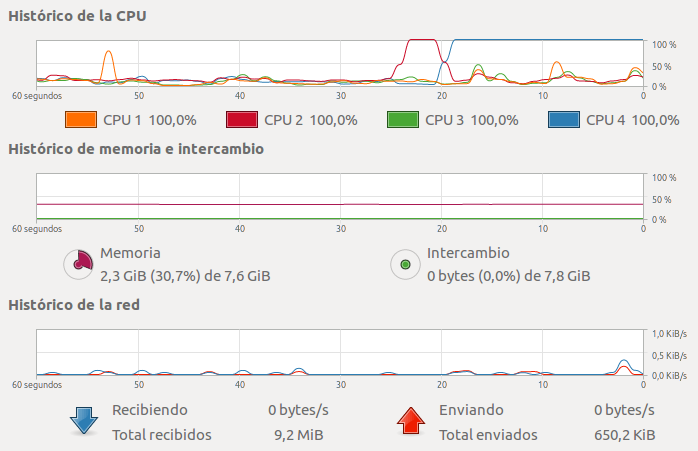
\includegraphics[scale=0.5]{../images/5.png}
	\caption{Inicio parte concurrente}
\end{figure}
\begin{figure}[h]
	\centering
	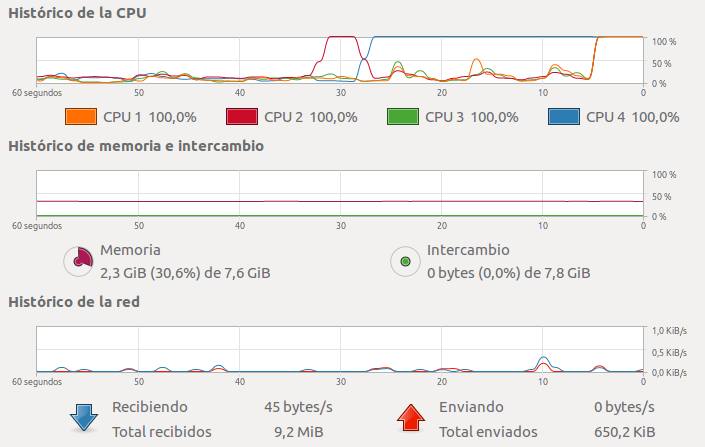
\includegraphics[scale=0.5]{../images/6.png}
	\caption{Parte concurrente}
\end{figure}
\begin{figure}[h]
	\centering
	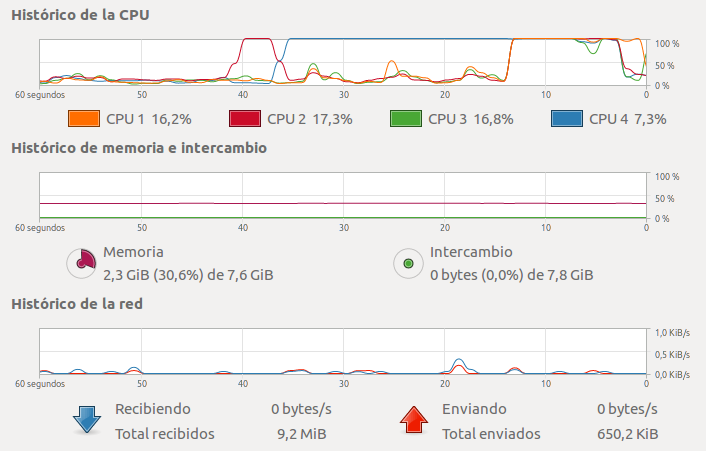
\includegraphics[scale=0.5]{../images/7.png}
	\caption{Finalización}
\end{figure}
\begin{figure}[h]
	\centering
	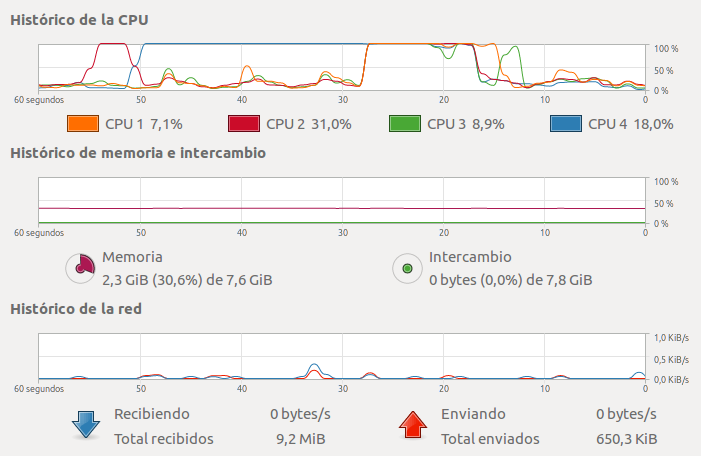
\includegraphics[scale=0.5]{../images/8.png}
	\caption{Histórico de lo que han hecho todas las hebras}
\end{figure}

Como bien se puede observar en las imágenes, al principio las CPUs están desocupadas, salvo la correspondiente a la hebra principal, en color azul, que ejecuta la versión secuencial en primer lugar, ocupando una CPU al cien por cien. Posteriormente, las cuatro hebras creadas por la principal pasan a ocupar cada una una CPU al 100\%, y la principal les espera, uniéndose una vez finalizado el cálculo.
\end{document}